\documentclass[12pt,twoside]{report}

%%%%%%%%%%%%%%%%%%%%%%%%%%%%%%%%%%%%%%%%%%%%%%%%%%%%%%%%%%%%%%%%%%%%%%%%%%%%%

% Definitions for the title page
% Edit these to provide the correct information
% e.g. \newcommand{\reportauthor}{Timothy Kimber}

\newcommand{\reporttitle}{Use of Deep Neural Networks for Visual Speech Decoding}
\newcommand{\reportauthor}{Alexandre Polise}
\newcommand{\supervisor}{Dr. Stavros Pitridis\\Dr. Maja Pantic}
\newcommand{\degreetype}{Computing Science}

%%%%%%%%%%%%%%%%%%%%%%%%%%%%%%%%%%%%%%%%%%%%%%%%%%%%%%%%%%%%%%%%%%%%%%%%%%%%%

% load some definitions and default packages
\input{includes}

% load some macros
\input{notation}

\date{September 2015}

\begin{document}

% load title page
\input{titlepage}


% page numbering etc.
\pagenumbering{roman}
\clearpage{\pagestyle{empty}\cleardoublepage}
\setcounter{page}{1}
\pagestyle{fancy}

%%%%%%%%%%%%%%%%%%%%%%%%%%%%%%%%%%%%
\begin{abstract}
Your abstract.
\end{abstract}

\cleardoublepage
%%%%%%%%%%%%%%%%%%%%%%%%%%%%%%%%%%%%
\section*{Acknowledgments}
Comment this out if not needed.

\clearpage{\pagestyle{empty}\cleardoublepage}

%%%%%%%%%%%%%%%%%%%%%%%%%%%%%%%%%%%%
%--- table of contents
\fancyhead[RE,LO]{\sffamily {Table of Contents}}
\tableofcontents 


\clearpage{\pagestyle{empty}\cleardoublepage}
\pagenumbering{arabic}
\setcounter{page}{1}
\fancyhead[LE,RO]{\slshape \rightmark}
\fancyhead[LO,RE]{\slshape \leftmark}

%%%%%%%%%%%%%%%%%%%%%%%%%%%%%%%%%%%%
\chapter{Introduction}
	\subsection{Motivation}
Recognising human speech is a task that is considered to be effortl	ess amongst human beings. Given knowledge of a language, understanding what is being spoken happens subconsciously [http://www.pnas.org/content/109/48/19614.abstract]. On the other hand, the same task requires complex algorithms and several steps of preprocessing in order for it to be performed by computers. 
\\ \\
The benefits of being able to program computers to understand spoken word are so great that much research has been performed in order to allow for speech recognition systems to develop to be usable and reliable. 
\\ \\
Traditional speech recognition systems are able to understand written and spoken word. Written word is normally processed by parsing visual written word into single-letter inputs, which can be passed through some detection algorithm which maps the written text to a written letter or number, usually a BLAH. Post-processing re-strings these single inputs together to make words, which can then form sentences. Audio data is processed and passed in through a similar method. Pre-processing involves segmenting audio data into single sounds, which can then be passed through a detection algorithm which maps them to a phoneme. These phonemes are strung together to form words. Through these methods, speech recognition can be used to sort mail, filter telephone calls, and myriad of other low level sorting processes that were once performed by humans. 
\\ \\
New approaches are being developed in order to process and understand spoken word via visual data. With the addition of a system that can detect what is being said through video input, videos with distorted or absent sound accompaniment can still be ‘understood’ by computer systems. 

	\subsection{Objectives}
The core objective is to train a neural network to recognise speech based on video input of humans speaking. This object will require the completion of several sub-objectives: 

\begin{enumerate}
	\item Data Acquisition and Pre-processing: Video data must be found which has the right and relevant information for this task. Furthermore, it must be preprocessed in a way such that it is labelled to be one speech sound and not another.
	\item Data compression:  Video data can be very large due to a sizeable number of frames, nearing one-hundred in high quality videos. Therefore, the video data must be compressed into be a size small enough to fit through a neural network. This can be performed in a number of ways, which are detailed below. 
	\item Neural Network Training: The data will then need to be passed through a neural network classifier, which will attempt to identify speech sounds based on input. Through several iterations, a large number of parameters can be adjusted to improve the performance of the network. These parameters can affect both time and accuracy.

\end{enumerate}

	\subsection{Contributions}
	\subsection{Report Outline}
Chapter 2: Presents some background history and a brief introduction into the use and functionality of neural networks and speech detection systems. \par
Chapter 3: Provides information on the choices made regarding data use, limitations of the data used, and pre-processing techniques tried and used on data. \par
Chapter 4: Presents the neural network being used, and the functionality that it provides. \par
Chapter 5: Presents the feature extraction algorithm used, and the functionality that it provides. \par
Chapter 6: Use of Autoencoder, results, parameters changed \par
Chapter 7: Classifier use, parameters changed, results \par
Chapter 8: Analysis of results, limitations, modifications and improvements that could be made, future research and conclusions \par
	
		
\begin{figure}[tb]
\centering

\includegraphics[width = 0.4\hsize]{./figures/imperial}
\caption{Imperial College Logo. It's nice blue, and the font is quite stylish. But you can choose a different one if you don't like it.}
\label{fig:logo}
\end{figure}


%%%%%%%%%%%%%%%%%%%%%%%%%%%%%%%%%%%%
\chapter{Background}
	\section{Neural Networks}
		\subsection{Historical Context}

Artificial neural networks (ANNs) can be defined as models that are able to perform highly discriminatory tasks via a dense interconnection of simple computational elements (Lippman, 1987). The structure of an artificial neural network is inspired by the human nervous system; ANNs have an inner layer of inputs, an outer layer of outputs, and some number of hidden layers, which receive input and send output but are not ‘seen’ by external users. Deep neural networks (DNN) is a term used to refer to networks who have more than one hidden layer. 
McCulloch and Pitts (1943) were the first to present some version of a neural network. This system was modelled directly after biological networks, and attempted to perform computational tasks using circuit logic. These tasks were completed using a very simplistic artificial neuron called a perceptron. Perceptrons can take in any number of inputs, and produce a single, binary output signal. 
\\ \\
Rosenblatt (1958) devised this neuron that computes its output by consulting weights, which are real numbers that clarify the relative importance of a given input to the output. If the summation of a given neuron’s weighted inputs passed the node’s threshold value, the neuron would ‘fire’, outputting a 1. Otherwise, it would output a 0. Perceptrons can express a multitude of different logical conditions, but are limited in that changing the weights of a single neuron, or node, can lead to grave differences in an entire neural network. This is due to the binary, ‘all-or-nothing’ nature of perceptrons.
\\ \\
Another, more commonly used, type of artificial neuron is the sigmoid neuron, whose nature is nearly identical to that of the perceptron, except that it’s output can be any numerical value between 0 and 1. 


		
\begin{figure}[tb]
\centering
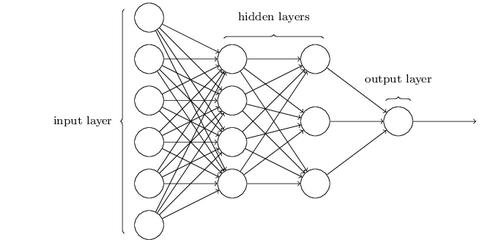
\includegraphics[width = 0.8\hsize]{./figures/neuralnet}
\caption{Example of a deep neural network (Nielsen, 2015).}
\label{fig:neuralnet}
\end{figure}



		\subsection{Supervised vs Unsupervised Networks}
		\subsection{Performance}
Neural networks are remarkably able to extract meaningful patterns from imprecise or complicated data that could not be well understood by humans or via the use of other computer techniques. (a) This is because a neural network is trained by example, and does not need to be told how to perform, but rather uses its network of interconnected neurons to learn patterns in a way that is meaningful to the network. In this way, neural networks are able to process data that is far more complex than traditional algorithmic approaches. But, training a neural network can leave a programmer feeling uncertain; it is not clear how a neural network works, or what it is doing, leaving the process of refining and improvements difficult.
\\ \\
	Neural networks can be feed-forward only, or can include loops, and can be unsupervised or supervised, where supervised learning insinuates that the neural network is told ‘the answer’ to several training examples. Some complexity arises when working with neural networks. For instance, data must be appropriately segmented before it is passed into a neural network. As an example, a neural network that identifies that value of written digits does not inherently know when one digit begins and another digit ends. Parsing the data so that the network can appropriately assess it is called ‘the segmentation problem’. 
\\ \\
Secondly, neural networks can be overtrained, leaving the network to ‘memorize’ training data and leave it unable to see similarities between very similar data. Overfitting is due to having high variance, which is error caused by having high sensitivity to very small fluctuations in the datasets. In order to decrease the chance of overfitting, weights can be penalized in proportion to their magnitude, or monitoring of learning can lead learning to stop early so that optimal performance is reached. (9) On the other hand, neural networks can be undertrained. An undertrained neural network is said to be underfit; it has not successfully developed a set of parameters by which differentiate each piece of data. An underfit neural network is so because of bias, error from incorrect assumptions in the learning algorithm (cite). In machine learning, finding balance between under and over-fitting data is describes ad the bias-variance tradeoff.
\\ \\	
Finally, the utility of a neural network comes from it’s ability to ‘learn’ through a succession of weight changes. But, given some input, it is not clear how weights should be changed throughout an entire neural network. This is because each node relies on information that it has been passed from an earlier node. Therefore, the weight change for a single node is not dependently only on itself and it’s own activity. 


		\subsection{The Backpropagation Algorithm}
Neural networks are trained by adjustments to the weights of each neuron in a way that reduces the error between the desired and actual output (a). This difference is known as the error derivative of the weights, and is most commonly computed using the backpropagation algorithm. Largely developed by Bryson, et al  (1963), (For descriptions, see (Haykin, 1991), (Kalman, 1960). Rumelhart, et al (1985) developed a clear explanation of backpropagation for networks where the error gradient of a node can be determined with only local information. Backpropagation minimises each node’s error using gradient descent and the least mean squares (LMS) algorithm. 


\begin{figure}[tb]
\centering
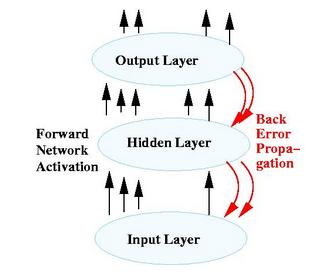
\includegraphics[width = 0.5\hsize]{./figures/backpropagation}
\caption{Animation of Backpropagation (Kerber, 2004).}
\label{fig:backpropagation}
\end{figure}



	Starting at the output layer, the EA is computed for each neuron, which is the rate at which the error changes as the activity level of a unit is changed (EW) (b). For the output layer, this is simply the LMS. Then, the algorithm moves one layer in, and computes the EA for the last hidden layer. This computation requires the algorithm to identify all of the weights between the hidden and output units that connect to it. (a) Those weights are multiplied by the EA’s of those units, and the products are added. The final sum is the EA for a neuron. 
	MATH
This process happens layer by layer, moving in the opposite direction that the network flows. From the EA, the EW can be computed; it is the product of the EA and the activity through the incoming connection. The EW is then used to adjust the weights of each individual neuron. Backpropagation over several iterations of training examples allows a network to fine tune its weights for the input that it is given.
MATH?

		\subsection{Experimentation and Results}

Neural networks’ use is widespread; industry applications range from stock market predictions to self-driving cars to presenting cardiopulmonary diagnostics. In the field of language recognition, neural networks have been used to perform written digit recognition (Cireşan, et al, 2010) (There are so many more citations for this, ask about what to do). Sigmoidal networks have been trained to detect handwritten digits and text {mmdl hinton \& salakhutdinov, salakhutdinov and hinton}. Deep neural networks have also been developed for large vocabulary continuous speech recognition systems (LVCSR) (Dahl, et al, 2013), natural language processing (Collobert, et al, 2008), and image classification (Krizhevsky, et al, 2012)). 
\\ \\
	The first speech recognition system was built in 1952 by Davis, et al(13) at Bell, Laboratories. The name of the system was Audrey, and it could only recognise digits 0-9. The field of speech recognition has since improved, and now many systems are trained to not recognize whole words, but rather recognize individual phonemes. While many databases have been used for speech recognition in the past, the TIMIT database has been extensively used. It is a large data set including American speakers from both genders speaking a variety of different English words. A review of the successes that individual systems have had in phoneme detection using the TIMIT database can be seen below. 
	\subsection{Hidden Markov Models}
Many of the previously successful speech recognition systems have had their basis in Hidden Markov Models (HMMs). Hidden Markov Models are popular for speech recognition because they allow context to play a part in a computer system. Without such context and dependency on previous data, speech recognition would be very difficult to perform, as human speech is highly context dependent, and many speakers co-articulate; that is, the sounds that they have previously said affect the way they say current sounds. Hidden Markov Models, developed by Rabiner (70) only use the last state as information when making decisions about a current state reducing the complexity of the problem. A Hidden Markov Model is based on the idea of a Markov Chain, which computes the probability of a present state given just the last state. 


Pr(St+1 = sjS1 = s1; S2 = s2; :::; St = st) = Pr(St+1 = sjSt = st)

This is done with the help of a state transition matrix, which gives the probability of any state coming after any other state. It also makes use of the initial probability of being in any given state. (e) 
\\ \\
An HMM is a Markov Chain where each state transition outputs an associated probability. This state probability combination is similar to a Markov Chain, in that a state causing a probability output requires the same dependencies as two independent states following one another. These probabilities build up over time, allowing a system to recognise the most likely series of state transitions.(e)

	\section{Computer Speech Recognition}
		\subsection{Acoustic Speech Recognition}

Speech is highly variable, but HMMs can be used to map out the state transition probabilities for a given language reasonably well (cite). This is because speech is made up of discrete chunks of information. In acoustic speech, phonemes have been described as being described by Gimson as ``The smallest contrastive linguistic unit which may bring about a change of meaning’’.[27] Phonemes and phones differ in that phones are sounds of a language, but phonemes convey an associated meaning. (e) 
\\ \\
The act of decoding what is being spoken through processing audio data is called Acoustic Speech Recognition, and it is of great interest to this project. While visual speech decoding is fairly new and therefore fairly undeveloped, high-performing acoustic speech recognitions exist and are used extensively in industry across several different platforms, including but not limited to translation websites and applications, hand-less GPS devices, and automatic typing machines (cite all 3). The development of more usable and reliable auditory speech recognition systems has propagated further research on the topic, and has led to research on visual speech recognition. 

	\subsection{Past Experimental Results}
Most acoustic speech recognition systems are built using XYZ. Their performance is XYZ.

		\subsection{Visual Speech Recognition}
Visual speech recognition, the act of recognizing what is being said using only visual cues, has entered the spotlight in recent years. The recent focus on improving visual speech recognition is largely so that these systems can be used in conjunction with other speech recognition systems. (Petajan, 1984).
\\ \\
Visual speech recognition could oftentimes fill the gap in data where audio speech recognition cannot be used. Data that is distorted, or where sound information isn’t reliable due to other noises or distractions, don’t fare well when being passed into an auditory speech recognition system, and in these instances visual speech recognition can be particularly useful  (Potamianos, et al, 2001). (cite) Furthermore, video data that does not come with any audio data cannot be processed at all by these audio recognition systems. 
\\ \\
It is these instances where visual speech recognition could assist audio speech recognition systems or work entirely independently in order to increase the amount of information extracted from a dataset. In this way, visual speech recognition can improve the accuracy of a computer systems computation of video and audio data in multimodal systems. (Adjoudani, et al, 1996), (Heckmann, et al, 2001), 

		\subsection{Visemes}
Both audio and visual speech recognitions gather a lot of their insight and information from the field of linguistics. Where many audio speech recognition systems use the phoneme, the smallest unit of sound, as the input of neural networks learning auditory cues, visual speech recognition systems have developed a similar unit, called a viseme. A viseme is a unit of visual data. There are several different definitions of a vieme, as is mentioned in Cappelletta (7 in tcdtimit), and unfortunately because of this, there is no uniform way of approaching or working with visemes. 
\\ \\
One definition includes all articulatory gestures into the definition of a viseme. That is, when a word or sound of a word is spoken, the summation of all visual cues, including the lips, teeth exposure, and the placement of the tongue, all create what is considered a viseme. Another definition maps visemes directly onto already extensively studied and reported phonemes, of which there is a decided and finite quantity (cite eoin). Using a mapping from visemes to phonemes means that there will be several phonemes that map to the same viseme. That is, the mapping will not be 1:1. This is because there are several sounds that can be made using the exact same visual appearance. An example of this would be /p/ and /d/, where the only difference between the two phonemes is that one is voiced and the other is voiceless. 

\begin{figure}[tb]
\centering
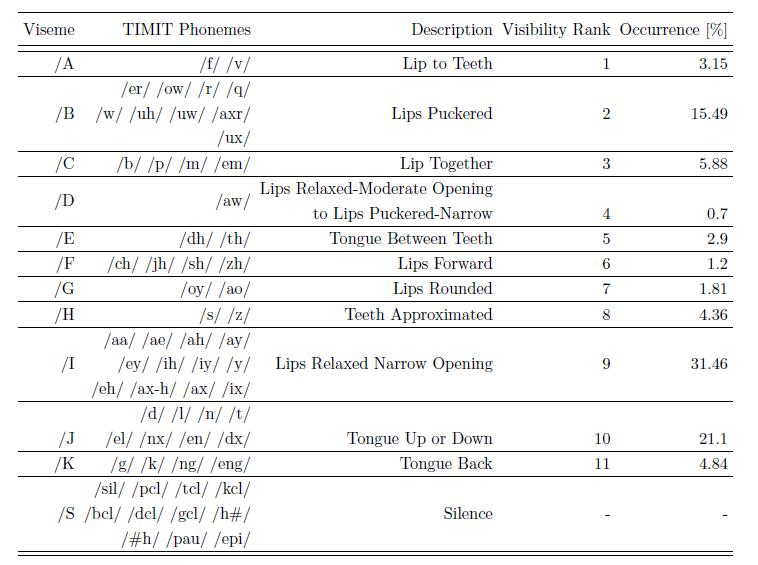
\includegraphics[width = 1.0\hsize]{./figures/jeffersbarleyvisememap}
\caption{Jeffers and Barley Phoneme-to-Viseme Map(Gillen, 2014).}
\label{fig:logo}
\end{figure}


		\subsection{Humans and Lipreading}
While the task of using visemes to discern what is being said is often referred to as ‘lipreading’, this name is misleading. It has been shown that physical cues from not only the lips, but also the face and tongue, play a role in this visual decoding process. (cite) And while those who are hard-of-hearing rely more heavily on visemes in order to understand spoken word (Bernstein, et al, 1998), the information is used, at least somewhat, by all humans, especially in situations where there is sound interference. for review, see (Summerfield, 1987) (Massaro, 1987)), In fact, even in non-noisy environments, speech recognition performance is improved when there is some visual information about the speaker present [5;http://ieeexplore.ieee.org/stamp/stamp.jsp?tp=\&arnumber=865479].
\\ \\
Visemes can influence what is ‘heard’ in real world settings, as seen by the McGurk effect. (McGurk et al, 1976) For instance, when shown the a person mouthing the sound /ba/ and played the sound /ga/ simultaneously, people often mistake this as being the sound /da/. This shows that people use and, to some extent, rely on the visual motions that are made when communicating with one another. 

		\subsection{Tracking Techniques}
		\subsection{Established Visual Speech Recognition Methods}
In showing that humans rely on visual cues in order to ‘hear’ what is being said, the McGurk effect has offered reason to unveil a system that can visually decode speech. The first lipreading system was reported by Petajan (1984) (Potamianos, et al 2004). Since then, many systems have been developed for visual speech decoding (Duchnowski, et al, 1996, Meier, et al, 1996, Yuhas, et al, 1989). 
\\ \\
Recent lipreading systems have been developed making use of deep belief networks (DBNs) (Huang, et al, 2013), time delay neural networks (TDNN) (Lavagetto, 1997), neural network classifiers (Shin, et al, 2011), unsupervised random forest manifold alignment (RFMA) (Pei, et al 2013), and deep bottleneck feature learning schemes by use of an autoencoder (Sui, et al, 2015), 
\\ \\
Yuhas, et al (1989) developed a neural network which predicted the auditory signal made given some visual input. Duchnowski, et al (1994) and Meier, et al (1996) trained networks to model phonemes and visemes, and then combined the predictions in a phonetic layer to predict the spoken phoneme. Ngiam, et al made a multimodal deep network system that did not model phonemes or visemes, but instead built bimodal representations by modelling the correlations across learned shallow representations (Ngiam, et al 2011).

more lbp-top
. Recently, Ahonen et al. proposed a novel facial representation for face recognition from static images based on LBP features [34], [35]
		\subsection{Acoustic and Visual Speech Decoding Integration}
	\section{Autoencoders}
		\subsection{Autoencoder Theory}
An Autoencoder is a type of neural network used to allow a system to recognise lower-dimension, more efficient encodings of generally larger sets of data. Autoencoders are typically used for dimensionality-reduction. Autoencoding is based on theories involving Sparse coding, proposed by  Olshausen et al. [4] in 1996. Sparse coding describes a neural network which represents an input by a strong activation of relatively few neurons. 
\\ \\
Like a normal, feed-forward neural network, an autoencoder has an input layer X, an output layer Z, and some hidden layers. But, unlike a neural network, the output layer of an autoencoder has just as many nodes as the input layer. This is because the goal of an autoencoder is to take an input, map it onto a severely smaller set of nodes, and be able to reproduce the input as the output layer. In other words, the autoencoder is supposed to train itself to reproduce a given input, given a much smaller layer (sometimes called a ‘bottleneck layer’).
The goal of the autoencoder is to produce a hidden layer, Y, that is a distributed representation of the input layer, X, which is able to embody the main factors of variation in X. [f]
\\ \\
http://ufldl.stanford.edu/wiki/images/thumb/f/f9/Autoencoder636.png/400px-Autoencoder636.png make an image like this one 
A denoising autoencoder is a popular type of autoencoder, especially in the field of computer vision. (??) This is largely because of the preventative nature that a denoising autoencoder can have over overfitting. Denoising autoencoders have the same main goal; that is, they want to be able to create a much smaller, distributed representation, Y, of an input X, with which they can produce a ‘mirror’ reproduction, Z. Denoising autoencoders force a system to learn more seriously the vital features of an image, though, by corrupting the input, X, and forcing it to reproduce Z allthewhile. This way, the system cannot simply ‘memorize’ the correct output given an input. Rather, it must be able to recognize an input from it’s features. In some research, as many as half of the input values are set to zero. [g] Denoising autoencoders may also be stacked, consisting of several layers of denoising autoencoders. 

		\subsection{Autoencoder Use in Speech Decoding Systems}
	\section{Texture Recognition}
		\subsection{Theory}
Texture recognitions seeks to assign an unknown sample to one of a number of known texture classes. Texture recognition is one of several problems grouped under the domain ‘texture analysis’. Successful texture recognition can be used in a variety of fields, ranging from ground classification to document analysis. 

	While texture recognition is highly complicated and there are very few examples of successful texture recognition systems, texture recognition is regularly used by humans subconsciously. (2)  Studies in the field of vision psychology have found that humans use texture recognition to perform scene identification when other cues are not present, and especially when images are shown for only very brief periods of time. (3)

	Texture analysis systems take in an image, and output some textural features for the image, which can be in several different forms. These textural features are then used to classify the same or similar training images, which are assigned to a texture. Test images are then passed through a classifier, and a well formed system would properly classify the test images, putting them into the proper texture feature category.
\\ \\
	Texture analysis can be performed in four ways: statistically, geometrically, model-based and signal processing. (4) Statistical methods analyze the distribution of pixel intensities across an image, computing local features at each point in the image. The method can vary in complexity, either addressing just one, two, or several pixels at once. 
\\ \\
Local binary pattern operators, which this research project will use, combine the occurrence statistics of local microstructures of an image (1). Local Binary Pattern (LBP) recognition consists of looking at each local pixel, and comparing it to the eight pixels surrounding it. Each neighbour is given a binary value depending on if it’s value is greater or less than the center pixel’s value. The output of this computation is a histogram which reflects the number of neighbouring pixels that are of greater intensity than the center pixel.

		\subsection{Dynamic Texture Analysis}
Dynamic LBP makes use of dynamic texture analysis, which is texture analysis on dynamic and changing image sequences. Previous work on classifying dynamic textures have been rooted in concatenating frames of the same video sequence and using hidden Markov models, or by use of optical flow or other spatio-temporal features. Dynamic LBP combines the local binary patterns with temporal information. 

\begin{figure}[tb]
\centering
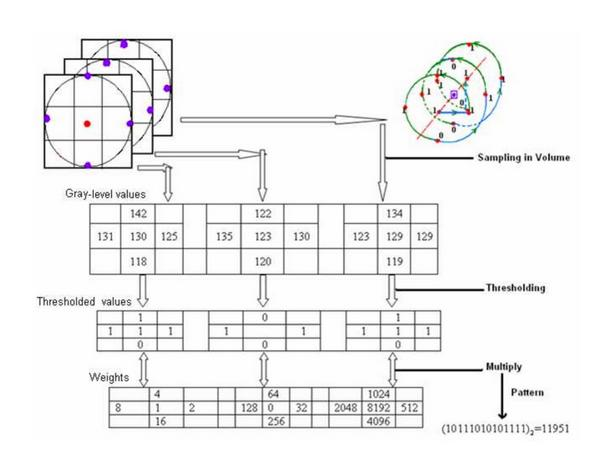
\includegraphics[width = 1.0\hsize]{./figures/VLBPprocedure}
\caption{ Procedure of V LBP1,4,1 ..}
\label{fig:logo}
\end{figure}


VLBP, basic dynamic LBP introduces a dynamic texture, V into the local neighbourhood of points surrounding a pixel. It takes in a series of temporally-relevant images, as the pixel in the same place as the center pixel from preceding and following frames are added to the neighbourhood and taken into account. The output of VLBP is a feature histogram of size (3P+2), where P is the number of neighbouring pixel points around the central pixel. 
\\ \\
VLBP computes a highly discriminative histogram, which increases in size as the number of features, P, increases. If the value of P becomes too large, the size of the resulting VLBP histogram can become overwhelmingly large, as an output histogram is 23P+2 in length.
Figure: Histogram
\\ \\
Texture descriptors have been successfully used for image recognition, and are often used because of their ability to function despite varying light intensities and and pose changes. (8) Local binary patterns have been successfully used in static image detection by dividing an image into several different sections, acquire LBP feature histograms for each, and concatenating them into a long feature vector. (9,10) In this way, most feature extraction experiments have been performed on static images. (11,12,13) Even facial expression analysis is usually performed on static images, extracting features in images that are seen to be the climax of expression for any given facial expression (happy, sad, angry). (14,15)

		\subsection{Texture Analysis Experimentation and Results}
The authors (8) of LBP-TOP propose a region concatenated descriptor for expression recognition of video data. Dividing the image into 8x9 blocks allows a feature detector to detect the location of micro-patterns, something that it is unable to do when passed in an entire image. The authors conclude that a region concatenated LBP-TOP feature vector can produce remarkable levels of recognition in classification systems, with classification levels reaching upper 90% success rates for most expressions. (8)
\\ \\
	Other experiments using LBP-TOP show similar success. Mattivi and Shao use LBP-TOP to perform human action recognition.(16)



%%%%%%%%%%%%%%%%%%%%%%%%%%%%%%%%%%%%
\chapter{Experimental Design}
	\section{Neural Network Toolbox}
		\subsection{Starting Parameters}
	\section{Choosing a Dataset}
In general, it is difficult to produce a helpful and adequate dataset for visual recognition experiments. Hundred-framed videos consisting of thousand or more pixel images creates a massive store of data. It is not clear which part of this data is essential, and large amounts of pre-processing and experimentation must be performed in order to extract the valuable or relevant data from these videos. Furthermore, experimentations in the field of speech recognition require an equal and consistent number of phrases to be spoken by a wide-enough group of people, preferably under different lighting conditions or from different angles. This variation would allow a system to avoid underfitting. 
\\ \\
For this reason, there are a limited number of databases available and suitable for this research project. In order for this research project to be carried out, it must make use of a database which:

\begin{enumerate}
	\item Has publically available, high-quality video data.
	\item Involves a relatively large number of different speakers.
	\item Ensures that the speakers speak a uniform yet varied number of spoken speech sounds.
	\item Is in spoken English.
\end{enumerate}

It would also be valuable if the database:
\begin{enumerate}
	\item Organized the videos by sounds spoken, or
	\item Included a mapping of phonemes or visemes.
	\item Was a suitable size for the scope and abilities of this project.
	\item Was easily segmentable into different speech sounds.
	\item Included videos or was comprised of videos that focused on the speaker's lips.
\end{enumerate}

Several databases were available for use, namely GRID, VidTIMIT, TCD-TIMIT, which had some to many of the required components. VidTIMIT [7] is an audio-visual database which involves 43 participants speaking 10 short sentences each. GRID is a similar database involving 24 speakers speaking a total of 1,000 sentences. VidTIMIT did not appear to have enough examples for a neural network, while GRID involved a much smaller vocabulary in its sentence choices. 

		\subsection{TCD-TIMIT Corpus}

The TCD-TIMIT corpus, developed by E. Gillen as part of a master’s thesis, is a very extensive audio-visual speech corpus that has 59 volunteers speakers video recorded at multiple angles speaking 98 sentences each, which are contained in approximately 150-framed 1920x1080-pixel videos. The database also includes video data for 3 professional lipspeakers, who say 377 sentences each. The videos are recorded at a rate of 30 frames per second. 
\\ \\
The database included both video data of the entire scene (a passport-style image of the speaker), as well as a video with only the mouth area (“region of interest”) 286x140 pixel-per-frame video included. This region of interest video data was very valuable, as it meant that less preprocessing would be required in order to pass the data through a network. The corpus included a speech-to-phoneme mapping of every utterance, which could be used to create a similar mapping to visemes, following a phoneme-to-viseme mapping chart such as the one shown earlier in this report. 
\\ \\
The creators of the database performed preliminary neural network experiments on the data, and inside of the master's thesis on the corpus, Gillen provided to extensive detail the split between train and test subjects, as well as other details involved in his research methods.

\begin{figure}[tb]
\centering
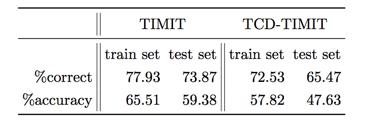
\includegraphics[width = 0.4\hsize]{./figures/tcdtimitaccuracy}
\caption{(Gillen, 2014)}
\label{fig:tcdtimit1}
\end{figure} 

Above are the results the TCD-TIMIT database produced for audio-only speaker-independent recognition in comparison with the TIMIT corpus off of which it was based. Results improved only marginally when the network was trained and tested on speaker-dependent test-train splits. 
\\ \\
Results on visual-only baseline experiments showed low accuracy in recognition overall, at 41% and 32% for correctness and accuracy, respectively.Gillen experimented with the number of Hidden Markov Model states (or layers), as well as the length of the input vector, which was varied by concatenating discrete cosine vector (DCT) vectors with their first and second derivatives. Gillen provided results by number of HMM states. Highest accuracy was found using 4-state HMMs, the accuracy details of which can be found in figure n.n.

\begin{figure}[tb]
\centering
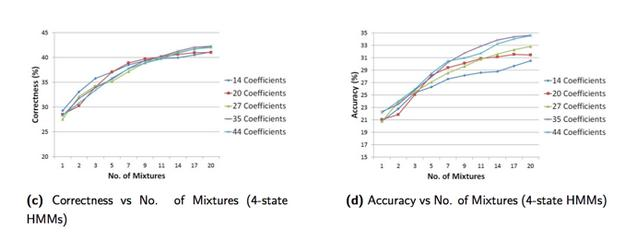
\includegraphics[width = 1.0\hsize]{./figures/correctnessoftcdtimit}
\caption{Highest Performance Visual-Only Experimental Results Using the TCD-TIMIT Database (Gillen, 2014)}
\label{fig:tcdtimit2}
\end{figure} 

Because of the high quality of the video data, as well as the plethora of resources provided for performing visual-only experiments using it, the TCD-TIMIT database was chosen as the database for this project.

		\subsection{Pre-processing of TCD-TIMIT Data}

Each video consisted of a single speaker speaking one sentence, which was comprised of approximately 40 phonemes. Therefore, each video needed to be parsed by viseme into separate videos, and then the correct viseme had to be mapped to the video file.
A video frame-to-phoneme mapping was given for each participant, for each video, which was a textfile with a start and end frame and a phoneme on each line. To begin pre-processing, a program (someprogram.m) to transform this per-frame phoneme mapping to a per-millisecond phoneme mapping was created. Next, a program had to be made that turned this phoneme mapping into a viseme mapping, by making use of a phoneme-to-viseme map, such as the mapping made by Potamianos, et al in the literature review of this report. A similar program was made in order to map each phoneme to a viseme (a number from 1 to 13). Because the mapping of phonemes to visemes is not 1:1, several phonemes were mapped to the same viseme. 
\\ \\
Next, each video needed to be parsed by video frame. A program called ``parse\_videos\_by\_viseme.m'' was created to perform this task. This program took in a video, and sorted the relevant frames for each viseme into separate cells of a cell array. Because the data available for each viseme was large (several frames long), further pre-processing had to be The use of a stacked autoencoder to extract features was chosen because of it’s success in providing more compressed and still successful data for similar recognition experiments [y].
Following the procedure of previous experiments using autoencoders [cite], the per-viseme videos were split up into 2x5 blocks, 4,004 pixels each, which were to be passed into the autoencoder individually. The final product would be a feature vector that consisted of the bottleneck layer (300 pixels) of each of these blocks concatenated together, resulting in a 3,000 element-long feature vector.  WAS THIS DONE O??
\\ \\
This data pre-processing was performed on only the ROI videos of one participant, the size of which was more than 4 GB. This amount of data is not allowed to be downloaded at once on a DoC computer, and took over an hour to download on a personal computer connected to high-speed wifi. In order to replicate the procedure that E Gillen followed for his experiments, it would take nearly 3 consecutive days of downloading, and over 250 GB of space, not accounting for space required to hold processed data. After proposing and rejecting several different solutions (acquiring a hard-drive, using only a subset of the data set), it was decided that, while the TCD-TIMIT dataset is ideal in many cases and should be used during a later part of this experiment, another dataset should be used before it so that some familiarity can be made with the neural network before performing such extensive work in pre-processing. 

		\subsection{The AV Letters Database}

Due to the massive amounts of unexpected pre-processing required, as well as severe space limitations, a smaller, more manageable database was opted midway through the project timeline. On this second approach to find an adequate database, several new constraints were enforced:

\begin{enumerate}
	\item Instead of finding a database with full sentence utterances contained in one video, a database where at most one word and at least one viseme were uttered would be preferred.
	\item Less types of utterances (26 possible utterances (ie, the alphabet), as opposed to ~50 different phonemes.
	\item A smaller set of data that can easily fit on the DoC computers without going over space limitations or restricting oneself to one machine.
\end{enumerate}

The AV letters database consists of 10 speakers (5 male, 5 female) producing three spoken utterances of the alphabet each. Combined, this creates 780 utterances, recorded at 25 frames per second using a Macintosh Quadra 660 av 8-bit ‘grayscale’ mode. Audio was recorded alongside. Along with full video data, the dataset includes a 60x80 pixel region-of-interest, similar to the TCD-TIMIT database. 

\begin{figure}[tb]
\centering
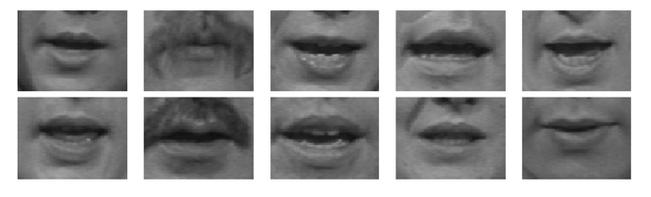
\includegraphics[width = 1.0\hsize]{./figures/exampleimagesavletters}
\caption{Example Data from the AV Letters Database (cite)}
\label{fig:avletters}
\end{figure} 

This database was labelled well, with each video taking the format: Letter-n-speaker, where Letter is one of the 26 letters of the English alphabet, n is the nth time this letter has been spoken by this speaker, and speaker is, naturally, the name of the person doing the speaking. 
\\ \\
The creators of the AV letters database performed myriad experiments on their own database, sampling different extraction methods (top-down versus bottom-up) in order to compare them all on an even playing field on the same continuous density Hidden Markov Model [87]. Results were found using a compressed (40x30) version of the video data recorded, and of all of the feature extraction methods, they found best results with the talker-independent shape model with per-talker GLDMs, at 41.9 percent accuracy.

\begin{figure}[tb]
\centering
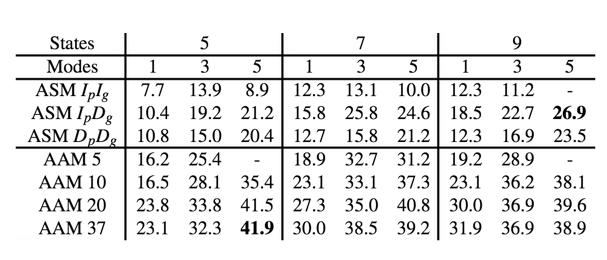
\includegraphics[width = 0.6\hsize]{./figures/avlettersaccuracy}
\caption{Recognition Accuracy Using the AV Letters Database with Various HMM States and Gaussian Models (cite)}
\label{fig:avletters2}
\end{figure} 

While their accuracy results for visual-only experiments were low, their visual only system, when integrated with their audio-only system, produced better results than either of the systems produced alone.

\begin{figure}[tb]
\centering
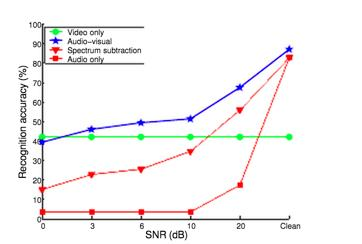
\includegraphics[width = 0.6\hsize]{./figures/accuracychartavletters}
\caption{Accuacy trends with visual only, audio only, audio-visul and spectrum subtraction data.  (cite)}
\label{fig:avletters2}
\end{figure} 

In comparison to the N number of videos in the TCD-TIMIT corpus, the 780 videos in the AV letters database is substantially less. The entire database was easily held on DoC computers, as well as the researcher's’ own personal computer, which made performing research less troublesome. While the number of speakers will allow for less experimentation, the AV letters database was chosen as a new starting point so that the rest of the project would be able to progress more smoothly.

The AV letters database, as mentioned above, is organized into separate videos by word. For the first series of experiments, which will not pre-process the data in order to take into account any temporal information, single frames will be passed in and will teach the neural network. Therefore, very little pre-processing had to be done in order to prepare the data for this experiment. In order to check the validity and accuracy of the neural network, some general guidelines will be followed: 

\begin{enumerate}
\item Every 60x80 (1x4,800) pixel frame will be passed in separately and stand as an input.
\item Each frame will not be passed in a way that suggest that it is related to the preceding and following frames. 
\item For purposes of the neural network classifier, the output value (y value) assigned to a frame (x value) will be a 1x26 long vector of zeros, with a ‘1’ at the position of the letter that it represents (ie, a ‘1’ at position 1 would signify that a frame is from an ‘A’ video). 
\item The frames of a single video will be passed in consecutively. This is to ensure that they are all kept together so that they can potentially be analysed as a group as well as single entities. 
\end{enumerate}

This methodology makes it easy to see which frames are more likely to be output with the correct response, which could make augmenting pre-discussed or creating new experiments easy and intuitive. For instance, if the first frame is generally guessed incorrectly, it would make sense to perform an experiment where each video was passed in without the first frame. 
\\ \\
The AV letters database was divided up into training, test, and validation sections. The division was speaker-independent; no speaker appeared in more than one set. The training set was comprised of the , while the validation set was comprised of the videos, and the test set was comprised of the videos. 

		\subsection{Dynamic Texture Analysis}
		
Dynamic texture analysis has been used in systems for performing texture analysis [4], facial expression recognition [4], emotion recognition[3],  human action recognition[1], and face biometrics recognition[2]. 
\\ \\
Feature extraction by use of dynamic texture analysis was chosen to be a part of this project because of the inherent temporal nature of the data being used. LBP-TOP was chosen as the dynamic texture analysis tool for this project because it has previously been used to detect differences in human faces [4]. The authors of LBP-TOP used the feature histogram in order to perform facial image analysis. As mentioned in the background section of this report, LBP-TOP takes in a matrix of grayscale image data points, and produces a feature histogram from these points. For computational simplicity, the authors of LBP-TOP concatenate local binary patterns on three orthogonal planes (LBP-TOP), and use only these planes when performing co-occurrence statistics. Several methods have been used to perform facial image analysis, including the use of optical flow [14], facial animation parameters [15], and a Tree-Augmented-Naive Bayes classifier[16]. But, these systems are either highly complex, or have low success rates using just a few subjects[4]. 
\\ \\
In order to increase recognition and decrease complexity, the authors of LBP-TOP proposed passing in sections of images to produce several, separate histograms that represent the texture of a specific place. Then, they proposed concatenating these feature histograms together, and using a classifier 

\begin{figure}[tb]
\centering
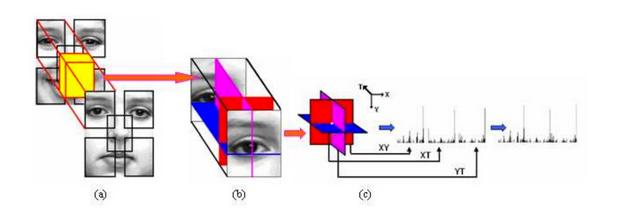
\includegraphics[width = 0.8\hsize]{./figures/lbptopprocess1}
\caption{Histograms are produced for several blocks of a series of frames [4]}
\label{fig:avletters2}
\end{figure} 

They chose to concatenate several histograms that represent only a portion of the overall image because a feature histogram that represents an entire video is only able to encode the micro-patterns of an image, and not the locations at which they reside [4]. The authors of LBP-TOP experimented with overlapping 4x3 blocks of an image, as well as non-overlapping 9x8 blocks. This experiment chose to begin analysis using non-overlapping 4x3 blocks, in order to reduce complexity. A P-value of size 8 was chosen, as the authors had best results with this value. 

\begin{figure}[tb]
\centering
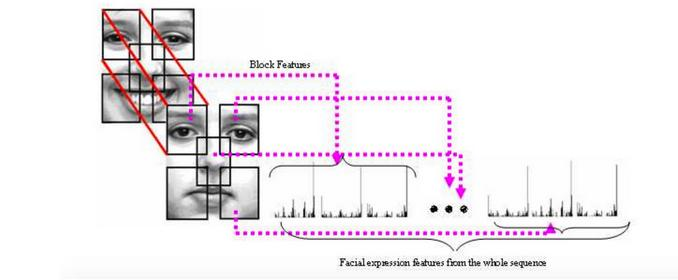
\includegraphics[width = 0.8\hsize]{./figures/lbptopprocess2}
\caption{The histograms of each block are then concatenated. [4]}
\label{fig:avletters2}
\end{figure} 

This project utilised the LBP-TOP Matlab files, provided by the authors [4]. The zipfile contains several helper functions, and a TEST\_VLBP\_LBPTOP.m file, which contains an example simple process for running LBP-TOP with a single video. This program was severely edited so that it could take in the large dataset of .mat files. The program also needed to be edited in order to take mxn blocks of a video and create separate histograms for each. 
\\ \\
Previous data preprocessing was used in order to separate the data into test, training and validation sets. The data was then split up into 4x3 non-overlapping blocks, and passed through a bespoke file that appropriately created histograms (of size 3x59) for each of the 12 blocks of every frame of every video, and saved them into .mat files. Post-processing was performed to concatenate the blocks into 1xN length feature vectors, which would be used as input values for classification. The output values assigned to these histograms are the same output values created for the plain pixel data, 1x26 long vectors of zeros, with a ‘1’ at the position of the letter that each histogram represents.


%%%%%%%%%%%%%%%%%%%%%%%%%%%%%%%%%%%%
\chapter{Data Manipulation}
	\section{Pre-processing}
	\section{Further Pre-processing}
	\section{Use of Dynamic Texture Analysis}
	\section{Compliance with Neural Network}



%%%%%%%%%%%%%%%%%%%%%%%%%%%%%%%%%%%%
\chapter{Training and Results}
	\section{Data Acquisition}
	\section{Test Results}
		\subsection{Autoencoder Results}


\begin{figure}[tb]
\centering
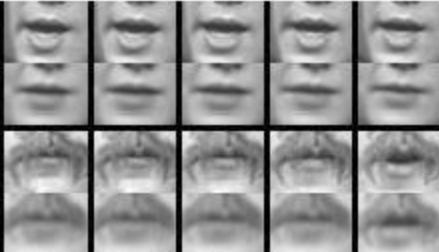
\includegraphics[width = 0.7\hsize]{./figures/sample_autoencode_results}
\caption{Sample output results when the AV Letters database was passed through an Autoencoder.}
\label{fig:logo}
\end{figure}

Figure~\ref{fig:logo} is an example of a figure. 



		\subsection{Increased Training Data Results}


%%%%%%%%%%%%%%%%%%%%%%%%%%%%%%%%%%%%
\chapter{Conclusion}
	\section{Evaluation}
	\section{Limitations}
	\section{Future Work}


%% bibliography
\bibliographystyle{apa}


\end{document}
